This chapter presents the results of this work. SNPs found in isolate series sampled from patients at the University Hospital of Basel are presented with available annotation. Furthermore, we demonstrate that the assembled morbidostat is very suitable for experimentally evolving resistance to cefepime with ESBL \textit{E. coli}. We also show SNPs in ESBL \textit{E. coli} strains potentially resulting from culturing with high antibiotic pressure.
\section{Identifying SNPs in ESBL \textit{E. coli} isolates series with changing cefepime susceptibility}
First, the phylogenetic tree will be presented that was used to ensure that all isolates of a series were the same strain and to show which isolates were selected for our analysis. Next will be shown which isolates of a series were chosen as a reference and as a last step the identified SNPs compared to the reference are shown. 
\subsection{Selection of isolate series suitable for our analysis}
\begin{figure}
	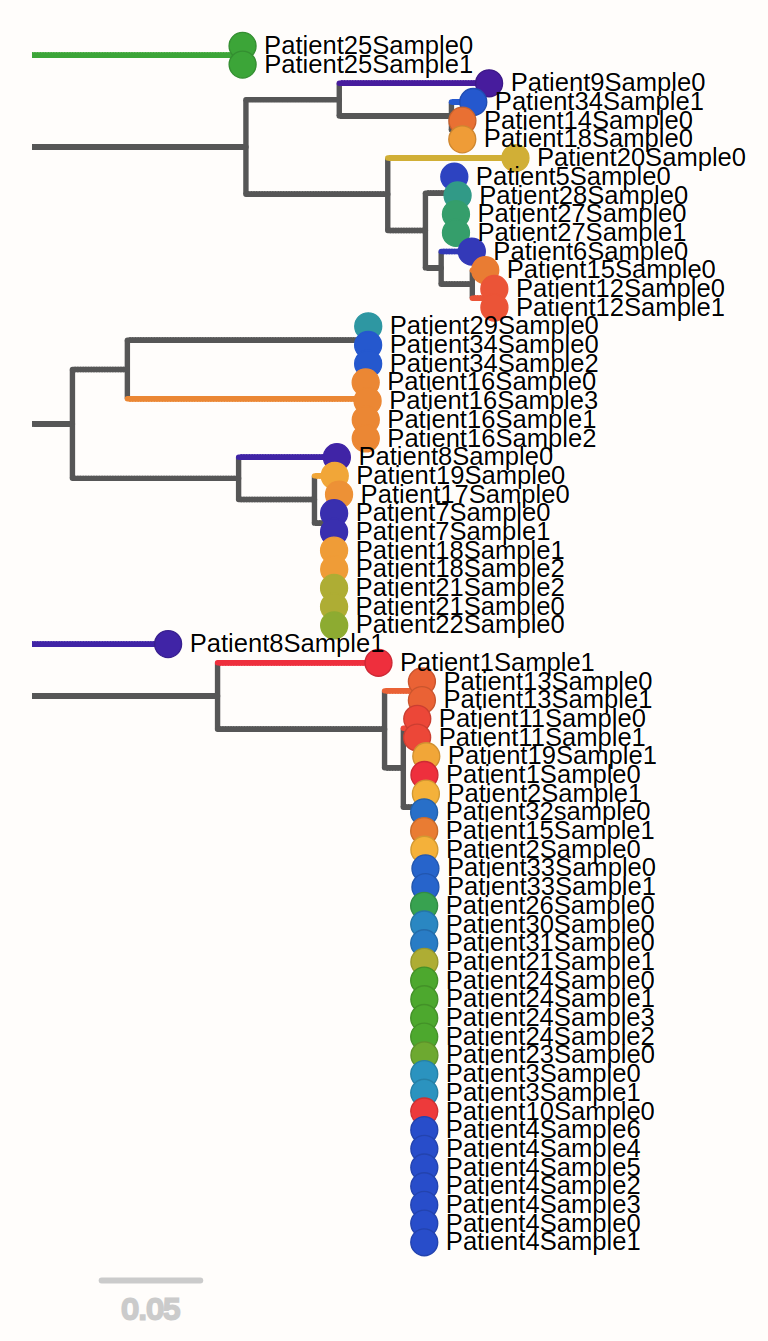
\includegraphics[scale=0.2]{181205_panXtree_overview.png}
	\caption{Phylogenetic tree built for every ESBL \textit{E. coli} isolate.}
	\label{figure:panX}
\end{figure}
We only included isolate series in our analysis with a significant change of the MICs over the sampling period and where all the isolates from a series were the same ESBL \textit{E. coli}. To ensure strain identity within a series we performed phylogenetic analysis with all isolates with panX \cite{ding_panx:_2018}.    
The phylogenetic tree of all isolates is shown in Figure \ref{figure:panX}. This tree revealed that many patients were infected with different ESBL \textit{E. coli} strains over time, suggesting reinfection rather than in-patient evolution. This is visible in the tree where isolates of one patient mapped on different branches. Interestingly some isolates from different patients mapped on the same branch which suggests that those patients were infected from the same outbreak. \\
We determined a change of the MICs as significant, if the MIC for cefepime increased at least by a factor of three. Applying the criteria of strain identity and significant change of MIC over the sampling period, five isolate series were left over. Those isolates and their MICs are shown in Table \ref{table:samples}.
\begin{table}
	\begin{tabularx}{\textwidth}{|cccLL|}
		\hline
		Patient                   & Isolate                   & Isolate date                     & MIC cefepime {[}\textmu g/mL{]} & MIC ceftazidime {[}\textmu g/mL{]} \\ \hline
		\rowcolor[HTML]{FFCE93} 
		{\color[HTML]{000000} 12} & {\color[HTML]{000000} 0} & {\color[HTML]{000000} 09/09/14} & {\color[HTML]{000000} 4}                      & {\color[HTML]{000000} 0.75}                       \\
		& 1                        & 05/12/14                        & 12                                            & 2                                                 \\ \hline
		\rowcolor[HTML]{FFCE93} 
		16                        & 0                        & 22/06/12                        & 8                                             & 2                                                 \\
		& 1                        & 18/07/13                        & 48                                            & 8                                                 \\
		& 2                        & 01/11/13                        & 32                                            & 12                                                \\ \hline
		\rowcolor[HTML]{FFCE93} 
		24                        & 0                        & 02/05/11                        & 4                                             & 1.5                                               \\
		& 1                        & 08/15/11                        & 16                                            & 1.5                                               \\
		& 2                        & 11/28/11                        & 3                                             & 1                                                 \\ \hline
		25                        & 0                        & 15/04/11                        & 64                                            & 192                                               \\
		\rowcolor[HTML]{FFCE93} 
		& 1                        & 22/08/11                        & 6                                             & 6                                                 \\ \hline
		33                        & 0                        & 26/09/14                        & 6                                             & 6                                                 \\
		\rowcolor[HTML]{FFCE93} 
		& 1                        & 29/01/15                        & 1                                             & 1.5                                               \\ \hline
	\end{tabularx}
	\caption{Selected ESBL \textit{E. coli} isolate series and their MIC of cefepime and ceftazidime. Isolates highlighted in orange were chosen as reference for the SNP analysis.}
	\label{table:samples}
\end{table}
\subsection{Identification of SNPs in patient isolates}
After selecting for isolate series suitable for our analysis we determined one isolate per series as a reference. We picked the isolate with the lowest MIC of cefepime as reference. If two isolates of a series had very similar MICs of cefepime (\textit{e.g.} isolate 0 and 2 from patient 24), we picked the isolate with the earlier sample date. The selected references of the series are stained orange in Table \ref{table:samples}. For the isolate series of patient 25 and 33 resistance decreased over the sample period. Therefore, the reference is isoalte 1, and not isolate 0 like for the other isolate series. From the selected references we hybrid-assembled their genome based on Illumina and ONT sequencing data. \\
We identified SNPs in the selected isolate series by comparing Illumina sequencing data of the isolates with emerged resistance to the genome of the reference of the series. We applied filtering of the SNPs by defining a minimal Illumina coverage of 30 at the position of the SNP. Additionally, only SNPs where the nucleotide in the isolates with emerged resistance changed in 80\% of the Illumina reads at this position compared to the reference will be presented.
\subsubsection{Isolate series of patient 12}
The isolate series of patient 12 consisted of two isolates sampled over three months. The EUCAST classifies strains with cefepime MICs bigger than 4 \textmu g/mL as resistant \cite{breakpoints}. The MIC of cefepime of isolate 0 was 4 \textmu g/mL and slightly below the breakpoint, but still very high. For this isolate series we identified two SNPs with no annotation. The SNPs are shown in Table \ref{table:patient12}.
\begin{table}
	\begin{tabularx}{\linewidth}{|cccLL|}
		\hline
		\#SNP & Contig & Position & \multicolumn{2}{l|}{Nucleotide in isolate:} \\
		&        &          & 0         & \multicolumn{1}{l|}{1}    \\ \hline
		1 & 0 & 880249  & C & A \\ \hline
		2 & 0 & 4256761 & A & T \\ \hline
	\end{tabularx}
	\caption{SNPs in the isolates of patient 12}
	\label{table:patient12}
\end{table} 
\subsubsection{Isolate series of patient 16}
From patient 16 three isolates were sampled over five months. The MICs of cefepime from every isolate exceeded the breakpoint. Therefore, all isolates were classified as resistant. Resistance advanced over the sample period visible in the MIC of cefepime of isoalte 1 which is 48 \textmu g/mL. We identified over 20 SNPs in the isolates of patient 16, but for only six genes annotation was available. Interestingly one SNP affected a promoter. The SNPs of the isolate series of patient 16 are shown in  Table \ref{table:patietn16}. The genes affected by the SNPs are shown in Table \ref{table:pat16annot} and the affected promoter in Table \ref{table:pat16_prom}.
\begin{table}[H]
	\begin{tabularx}{\linewidth}{|cccLLL|}
		\hline
		\#SNP & Contig & Position & \multicolumn{3}{l|}{Nucleotide in Isolate:} \\
		&        &          & 0     & 1     & \multicolumn{1}{l|}{2}    \\ \hline
		1     & 0      & 109928   & C     & A     & \multicolumn{1}{l|}{C}    \\ \hline
		2     & 0      & 1895312  & A     & C     & \multicolumn{1}{l|}{A}    \\ \hline
		3     & 0      & 2101128  & G     & -     & \multicolumn{1}{l|}{-}    \\ 
		&        & 2101129  & C     & -     & \multicolumn{1}{l|}{-}    \\ 
		&        & 2101130  & A     & -     & \multicolumn{1}{l|}{-}    \\ \hline
		4     & 0      & 2375277  & C     & T     & \multicolumn{1}{l|}{C}    \\ \hline
		5     & 0      & 3797984  & A     & G     & \multicolumn{1}{l|}{A}    \\ \hline
		6     & 0      & 4200032  & T     & C     & \multicolumn{1}{l|}{T}    \\ \hline
		7     & 0      & 4353560  & G     & C     & \multicolumn{1}{l|}{G}    \\ \hline
		8     & 0      & 5112127  & G     & T     & \multicolumn{1}{l|}{G}    \\ \hline
		9     & 0      & 55597    & A     & G     & \multicolumn{1}{l|}{G}    \\ \hline
		10    & 0      & 922702   & G     & A     & \multicolumn{1}{l|}{G}    \\ \hline
		11    & 0      & 1133762  & C     & T     & \multicolumn{1}{l|}{T}    \\ \hline
		12    & 0      & 1549518  & T     & G     & \multicolumn{1}{l|}{G}    \\ \hline
		13    & 0      & 2016331  & A     & C     & \multicolumn{1}{l|}{A}    \\ \hline
		14    & 0      & 2101129  & C     & -     & \multicolumn{1}{l|}{-}    \\ 
		&        & 2101130  & A     & -     & \multicolumn{1}{l|}{-}    \\ \hline
		15    & 0      & 3920934  & A     & G     & \multicolumn{1}{l|}{A}    \\ \hline
		16    & 0      & 4333944  & C     & T     & \multicolumn{1}{l|}{T}    \\ \hline
		17    & 0      & 4459680  & C     & -     & \multicolumn{1}{l|}{C}    \\ 
		&        & 4459681  & C     & -     & \multicolumn{1}{l|}{C}    \\ \hline
		18    & 0      & 4459684  & G     & -     & \multicolumn{1}{l|}{G}    \\ 
		&        & 4459685  & A     & -     & \multicolumn{1}{l|}{A}    \\ 
		&        & 4459686  & A     & -     & \multicolumn{1}{l|}{A}    \\ 
		&        & 4459687  & G     & -     & \multicolumn{1}{l|}{G}    \\ 
		&        & 4459688  & A     & -     & \multicolumn{1}{l|}{A}    \\ 
		&        & 4459689  & G     & -     & \multicolumn{1}{l|}{G}    \\ \hline
		19    & 0      & 4459692  & A     & -     & \multicolumn{1}{l|}{A}    \\ 
		&        & 4459693  & G     & -     & \multicolumn{1}{l|}{G}    \\ \hline
		20    & 0      & 4459695  & G     & -     & \multicolumn{1}{l|}{G}    \\ \hline
		21    & 0      & 4459697  & T     & -     & \multicolumn{1}{l|}{T}    \\ \hline
	\end{tabularx}
	\caption{SNPs in the isolates of patient 16.}
	\label{table:patietn16}
\end{table}
\begin{table}[H]
	\begin{tabular}{|lll|}
		\hline
		\#SNP & Transcription unit & Next upstream gene \\ \hline
		16    & fes-ybdZ-entF-fepE & \textit{fepA}      \\ \hline
	\end{tabular}
	\caption{Identified promoter affected by a SNP in the isolates of patient 16.}
	\label{table:pat16_prom}
\end{table}
\begin{table}
	\begin{tabularx}{\linewidth}{|ccLLccc|}
		\hline
		\#SNP & Gene          & Product                                  & Type and position in gene      & \multicolumn{3}{l|}{Amino acid in isolate:} \\
		&               &                                          &                        & 0   & 1               & 2               \\ \hline
		1     & \textit{ortT} & Orphan toxin OrtT                        & Missense, 44           & P   & T               & P               \\ \hline
		2     & \textit{scrY} & Sucrose Porin                            & Missense, 104          & L   & V               & L               \\ \hline
		3     & \textit{cpdA} & Phosphodiesterase CpdA                   & In-frame deletion, 162 & L   & -   & -   \\ \hline
		4     & \textit{rpoB} & DNA-directed RNA polymerase subunit beta & Missense, 113          & V   & I               & V               \\ \hline
		5     & \textit{ftsQ} & Cell division protein FtsQ               & Missense, 207          & K   & R               & K               \\ \hline
		4     & \textit{recR} & Recombination protein RecR               & Missense, 40           & M   & T               & M               \\ \hline
		5     & \textit{hcxA} & Hydoxycarboxylate dehydrogenase A        & Missense, 332          & R   & G               & R               \\ \hline
		6     & \textit{ribA} & GRP cyclohydrolase-2                     & Missense, 68           & F   & L               & L               \\ \hline
	\end{tabularx}
	\caption{Genes affected by SNPs found in the isolates of patient 16.}
	\label{table:pat16annot}  
\end{table}

The fepA promoter sequence affected by a SNP is shown in Figure 3.2. The polymorph position, marked with a red box, was found in the binding site of the \textsigma 70 transcription factor.  
\begin{texshade}{pat16fepa.aln}
	\showruler{1}{top}
		\feature{bottom}{1}{24..29}{fill:-}{-35}
	\feature{bottom}{1}{48..53}{fill:-}{-10}
	\feature{top}{1}{60..60}{fill:$\downarrow$}{Start of $\sigma$70 binding site}
	\hideconsensus
	\frameblock{1}{80..80}{Red[1pt]}
	\showcaption{This alignment shows the SNP in the fepA promotor. Positions marked with dashed lines are the recognition sites for $\sigma$70 factor.}	
\end{texshade}
\subsubsection{Isolate series of patient 24}
The isolate series of patient 24 consisted of three isolates. The MIC of cefepime from isolate 1 exceeded the breakpoint and was classified as resistant. For isolate 2 the resistance decreased again, and dropped below the breakpoint. Identified SNPs in the isolates of patient 24 are show in Table \ref{table:pat24}, the affected genes are shown in Table \ref{table:pat24_ann}.
\begin{table}
	\begin{tabularx}{\linewidth}{|cccLLL|}
		\hline
		\#SNP & Contig & Position & \multicolumn{3}{l|}{Nucleotide in isolate:} \\
			&        &          & 0     & 1     & \multicolumn{1}{l|}{2}    \\ \hline
	1     & 0      & 50032    & G            & A            & G            \\ \hline
	2     & 0      & 418564   & C            & T            & C            \\ \hline
	3     & 0      & 2048961  & A            & C            & C            \\ \hline
	4     & 0      & 2319554  & T            & A            & A            \\ \hline
	5     & 0      & 3444478  & T            & C            & T            \\ \hline
	6     & 0      & 4063226  & G            & T            & T            \\ \hline
	\end{tabularx}
	\caption{SNPs in the isolates of patient 24.}
	\label{table:pat24}
\end{table}

\begin{table}
	\begin{tabularx}{\linewidth}{|ccLLccc|}
		\hline
		\#SNP & Gene          & Product                                  & Type and position in gene      & \multicolumn{3}{l|}{Amino acid in isolate:} \\
		&               &                                          &                        & 0   & 1               & 2               \\ \hline
		1     & \textit{atl}     & DNA base-flipping protein                                  & Missense, 87      & V           & M           & V           \\ \hline
		2     & \textit{imm\_2}  & Colicin-E7 immunity protein                                & Missense, 69      & K           & E           & K           \\ \hline
		3     & \textit{lldR\_2} & Lactate Dehydrogenase regulatory protein & Missense, 44      & I           & S           & S           \\ \hline
		4     & \textit{dctM\_2} & TRAP transporter large permease protein                                                        & Missense, 112     & T           & S           & S           \\ \hline
		5     & \textit{dltA}    & D-alanine--D-alanyl carrier protein ligase subunit 1           & Missense, 692     & E           & G           & E           \\ \hline
		6     & \textit{fnr}     & Fumarate and nitrate reduction regulatory protein          & Missense, 31      & C           & F & F  \\ \hline    
	\end{tabularx}
	\caption{Genes affected by the SNPs found in the isolates of patient 24.}
	\label{table:pat24_ann}
\end{table}

\subsubsection{Isolate series of patient 25}
Two isolates were sampled from patient 25. Isolate 0 shows the highest cefepime MIC, which was 64 \textmu g/mL, of all selected isolates. In the case of patient 25 the resistance decreased over the sample period. Isolate 1, with a cefepime MIC of 6 \textmu g/mL was still classified as resistant. 
The identified SNPs between the isolates of patient 25 are shown in Table \ref{table:pat25}. The genes affected by those SNPs are shown in Table \ref{table:pat25_ann}.

\begin{table}
	\begin{tabularx}{\linewidth}{|cccLL|}
		\hline
		\#SNP & Contig & Position & \multicolumn{2}{l|}{Nucleotide in isolates:} \\
		&        &          & 0         & \multicolumn{1}{l|}{1}    \\ \hline
	1 & 0 & 396325   & G & A \\ \hline
	2 & 0 & 396846  & G & A \\ \hline
	3 & 0 & 1996537 & - & C \\ 
	&   & 1996538 & - & C \\ 
	&   & 1996539 & - & G \\ 
	&   & 1996540 & - & T \\ 
	&   & 1996541 & - & A \\ 
	&   & 1996542 & - & C \\ 
	&   & 1996543 & - & C \\ 
	&   & 1996544 & - & A \\ 
	&   & 1996545 & - & G \\ 
	&   & 1996546 & - & C \\ 
	&   & 1996547 & - & T \\ 
	&   & 1996548 & - & G \\ \hline
	4 & 0 & 3743644 & A & G \\ \hline
	5 & 0 & 4785433 & G & A \\ \hline
	6 & 0 & 4785439 & G & A \\ \hline
	\end{tabularx}
	\caption{SNPs in the isolates of patient 25.}
	\label{table:pat25}
\end{table} 

\begin{table}
	\begin{tabularx}{\linewidth}{|ccLLcc|}
		\hline
	\#SNP & Gene          & Product                                 & Type and position & \multicolumn{2}{l|}{Amino acid isolate:} \\
	&               &                                         &                   & 0                  & 1                  \\ \hline
	1     & \textit{ompR} & Transcriptional regulatory protein OmpR & Missense, 146     & R                  & H                  \\ \hline
	2     & \textit{envZ} & Osmolarity sensor protein EnvZ          & Missense, 84      & G                  & E                  \\ \hline
	3     & \textit{rfbD} & dTDP-4-dehydrorhamnose reductase        & \multicolumn{3}{l|}{Frameshift deletion, 148-295}            \\ \hline
	\end{tabularx}
	\caption{Genes affected by the SNPs found in the isolates of patient 25.}
	\label{table:pat25_ann}
\end{table}

\subsubsection{Isolate series of patient 33}
As for the series of patient 25, the resistance deceased in the isolates of patient 33. Isolate 0 was classified as resistant, while isolate 1 was classified as cefepime susceptible. Three SNPs were found in the isolates of patient 33, they are shown in Table \ref{table:pat33} with their annotation in Table \ref{table:pat33_ann}.
\begin{table}
	\begin{tabularx}{\linewidth}{|cccLL|}
		\hline
		\#SNP & Contig & Position & \multicolumn{2}{l|}{Nucleotide in isolate:} \\
		&        &          & 0         & \multicolumn{1}{l|}{1}    \\ \hline
		1 & 0 & 4008745 & A & T \\ \hline
		2 & 0 & 4675092 & T & A \\ \hline
		3 & 0 & 1996537 & A & C \\ \hline
	\end{tabularx}
	\caption{SNPs in the isolates of patient 33.}
	\label{table:pat33}
\end{table} 
\begin{table}
	\begin{tabularx}{\linewidth}{|ccLLcc|}
		\hline
		\#SNP & Gene          & Product                           & Type and position & \multicolumn{2}{l|}{Amino acid isolate:} \\
		&               &                                   &                   & 0                  & 1                  \\ \hline
		1     & \textit{cydD} & ATP-binding/permease protein CydD & Missense, 368     & Q                  & L                  \\ \hline
		2     & \textit{vnfA} & Nitrogen fixation protein VnfA    & Missense, 169     & N                  & I                  \\ \hline
	\end{tabularx}
	\caption{Genes affected by the SNPs found in the isolates of patient 33.}
	\label{table:pat33_ann}
\end{table}
\subsection{Copy numbers of ESBL genes}
We checked if the copy numbers of ESBL genes correlated with emerged resistance. Therefore, we analyzed the annotation of the hybrid-assembly of every isolate. Copy numbers of three ESBL genes of the selected isolates are shown in Table \ref{table:copynumers}. The copy number remained very similar for four out of five patients. Sometimes the ESBL gene was replaced by a different ESBL gene. Only the isolate series of patient 33 showed an increased copy number of ESBL genes while resistance was high, with the copy number decreasing as the resistance decreased. Isolate 0 of patient 33 had 9 copies of CTX-M-1 while isolate 1 only had one. 
\begin{table}
	\begin{tabularx}{\linewidth}{|ccLLL|}
		\hline
		Patient & Isolate & \multicolumn{3}{l|}{Copies of genes coding for \textbeta-lactamase} \\
		&        & CTX-M-1                & OXA-1                & TEM                \\ \hline
		12      & 0      & 1                      & 0                    & 0                  \\ \hline
		12      & 1      & 1                      & 0                    & 0                  \\ \hline
		16      & 0      & 2                      & 0                    & 1                  \\ \hline
		16      & 1      & 2                      & 0                    & 1                  \\ \hline
		16      & 2      & 1                      & 0                    & 1                  \\ \hline
		24      & 0      & 1                      & 0                    & 2                  \\ \hline
		24      & 1      & 1                      & 0                    & 2                  \\ \hline
		24      & 2      & 0                      & 0                    & 3                  \\ \hline
		25      & 0      & 1                      & 1                    & 0                  \\ \hline
		25      & 1      & 1                      & 1                    & 0                  \\ \hline
		33      & 0      & 9                      & 0                    & 1                  \\ \hline
		33      & 0      & 1                      & 1                    & 0                  \\ \hline		
	\end{tabularx}
	\label{table:copynumers}
	\caption{Copy number of ESBL genes per isolate.}
\end{table}

\section{Morbidostat experiments}
The experimental evolution of cefepime resistance with ESBL E. coli strains was successfully achieved by culturing with the morbidostat. Proof that resistance increased was obtained by comparing the MIC of cefepime from the strains before and after culturing with the morbidostat. \\
We performed two morbidostat experiments, experiment 01 and experiment 02. By culturing with the fixed\_OD with some vials we included controls where no antibiotic-pressure was applied to the strains. Table \ref{table:vial_modes} shows which ESBL \textit{E. coli} strain were cultured in which vial, with which mode. 
\begin{table}
	\begin{tabular}{|c c c c|}	
		\hline
		Vial & Strain ID & ESBL & Mode \\
		\hline
		1 & pEU26 & OXA-1 & Continuous \\
		\hline
		2 & pEU26 & OXA-1 & Continuous \\
		\hline
		3 & pEU23 & OXA-1 & Continuous \\
		\hline
		4 & pEU23 & OXA-1 & Continuous \\
		\hline
		5 & pEU23 & OXA-1 & Continuous \\
		\hline
		9 & pEU26 & OXA-1 & Continuous \\
		\hline
		10 & pEU23 & OXA-1 & Fixed OD \\
		\hline
	\end{tabular}
	\quad
	\begin{tabular}{|c c c c|}	
		\hline
		Vial & Strain ID & ESBL &Mode \\
		\hline
		1 & pEU26 & OXA-1 & Continuous \\
		\hline
		2 & pEU23 & OXA-1 & Continuous \\
		\hline
		3 & pEU22 & CTX-M-1 & Continuous \\
		\hline
		4 & pEU22 & CTX-M-1 & Continuous \\
		\hline
		5 & pEU22 & CTX-M-1 & Continuous \\
		\hline
		7 & K12 MG1655& None & Continuous \\
		\hline
		8 & pEU22 & CTX-M-1 & Fixed OD \\
		\hline
		9 & pEU26 & OXA-1 & Fixed OD \\
		\hline
		10 & pEU26 & OXA-1 & Fixed OD \\
		\hline
	\end{tabular}
	\caption{Left table: Used culturing mode and strains for experiment 01. Right table: Used culturing mode and strains for experiment 02.}
	\label{table:vial_modes}
\end{table}
\subsection{Contamination analysis}
For many samples we morphologically determined contaminations. Because we had Illumina sequecing data of every sample, we could determine the contamination as \textit{Bacillus cereus}. To ensure that the stocks of the strains were not contaminated, we mapped the Illumina data of the stocks to the hybrid-assembled \textit{E. coli} reference genome and \textit{Bacillus cereus} genome obtained from NCBI \cite{noauthor_bacillus_nodate}. The percentage of how many reads mapped to \textit{E. coli} and \textit{Bacillus cereus} is shown in Table \ref{table:bacillus_reads}. Around 0.44 \% of all Illumina reads mapped to \textit{Bacillus cereus} ATCC 14579. In Figure \ref{figure:bacillus_reads} one region of an alignment of the Illumina reads to the \textit{Bacillus cereus} genome is shown. It can be seen that the Illumina reads only mapped to very certain regions of the genome of \textit{Bacillus cereus} without overlapping and with a variation of a few bases. Because the reads were not overlapping and they did not map with an identity of 100\%, we concluded that the stocks were not contaminated. Also the hybrid-assembly of the reference genome did not show any contigs with \textit{Bacillus cereus} sequences. \\
We mapped the Illumina reads from the morbidostat samples to the hybrid-assembled \textit{E. coli} genome and the \textit{Bacillus cereus} genome in order to identify contaminated samples. The outcome is shown in Table \ref{table:bacillus_reads_samples}. Looking at the percentage of how many reads mapped to \textit{Bacillus cereus} showed that two groups exist. Either 60 \% or more mapped to \textit{Bacillus cereus}, implying that the samples were contaminated, or only 0.48\% mapped implying that those samples were not contaminated. From all morbidostat samples 12 samples had fewer reads than 0.48\% and were not contaminated.
\begin{table}[H]
	\begin{tabularx}{\linewidth}{|LLLLL|}
		\hline
		Stocked strain    & Total reads & Reads mapped to \textit{Bacillus cereus} & Reads mapped to \textit{E. coli} & \% of reads mapped to \textit{Bacillus cereus ATCC 14579} \\ \hline
		pEU22\_CTX & 3810442     & 16496                                                     & 3803789                                           & 0.43                                                            \\ \hline
		pEU23\_OXA & 4329090     & 18499                                                     & 4322708                                           & 0.43                                                            \\ \hline
		pEU26\_OXA & 4040571     & 17629                                                     & 4036167                                           & 0.44                                                            \\ \hline
		K-12 MG1655      & 4939319     & 21902                                                     & 4931214                                           & 0.44                                                            \\ \hline
	\end{tabularx}
	\caption{Illumina reads from every stock were mapped to a \textit{Bacillus cereus} genome from NCBI and the \textit{E.coli} reference genome produced with  hybrid-assembling \cite{noauthor_bacillus_nodate}.}
	\label{table:bacillus_reads}
\end{table}
\begin{table}[H]
	\begin{tabularx}{\linewidth}{|LccLLLL|}
		\hline
		Experiment & Vial & Sample & Total reads & Reads mapped to \textit{Bacillus cereus} & Reads mapped to \textit{E. coli} & \% of reads mapped to \textit{Bacillus cereus} \\ \hline
		01         & 1    & 1      & 6490750     & 4967611                         & 272289                  & 76.53                                \\ \hline
		01         & 2    & 1      & 7601839     & 6001106                         & 418578                  & 78.94                                \\ \hline
		01         & 3    & 1      & 2940556     & 13976                           & 2934902                 & 0.48                                 \\ \hline
		01         & 4    & 1      & 8167777     & 6150829                         & 281584                  & 75.31                                \\ \hline
		01         & 5    & 1      & 5606842     & 4089104                         & 178462                  & 72.93                                \\ \hline
		01         & 9    & 1      & 5636939     & 4466280                         & 268813                  & 79.23                                \\ \hline
		01         & 10   & 1      & 4935808     & 22368                           & 4928816                 & 0.45                                 \\ \hline
		02         & 1    & 1      & 6152378     & 26815                           & 6143228                 & 0.44                                 \\ \hline
		02         & 2    & 1      & 6926506     & 5180940                         & 291927                  & 74.80                                \\ \hline
		02         & 3    & 1      & 5142535     & 24909                           & 5136761                 & 0.48                                 \\ \hline
		02         & 3    & 2      & 6196309     & 4694898                         & 279679                  & 75.77                                \\ \hline
		02         & 4    & 1      & 4923087     & 22342                           & 4915639                 & 0.45                                 \\ \hline
		02         & 4    & 2      & 4589212     & 20628                           & 4582915                 & 0.45                                 \\ \hline
		02         & 5    & 1      & 4298753     & 17870                           & 4292083                 & 0.42                                 \\ \hline
		02         & 5    & 2      & 5189054     & 22772                           & 5181923                 & 0.44                                 \\ \hline
		02         & 7    & 1      & 5167596     & 22583                           & 5159028                 & 0.44                                 \\ \hline
		02         & 7    & 2      & 4976635     & 3015316                         & 107767                  & 60.59                                \\ \hline
		02         & 8    & 1      & 4356280     & 19067                           & 4350598                 & 0.44                                 \\ \hline
		02         & 8    & 2      & 4186125     & 18526                           & 4181356                 & 0.44                                 \\ \hline
		02         & 9    & 1      & 4182681     & 18487                           & 4176477                 & 0.44                                 \\ \hline
		02         & 10   & 1      & 3809536     & 2576863                         & 136340                  & 67.64                                \\ \hline
	\end{tabularx}
	\caption{Illumina reads from every morbidostat sample mapped to a \textit{Bacillus cereus} from NCBI and the \textit{E.coli} reference genome produced with  hybrid-assembling \cite{noauthor_bacillus_nodate}.}
	\label{table:bacillus_reads_samples}
\end{table}
\begin{figure}
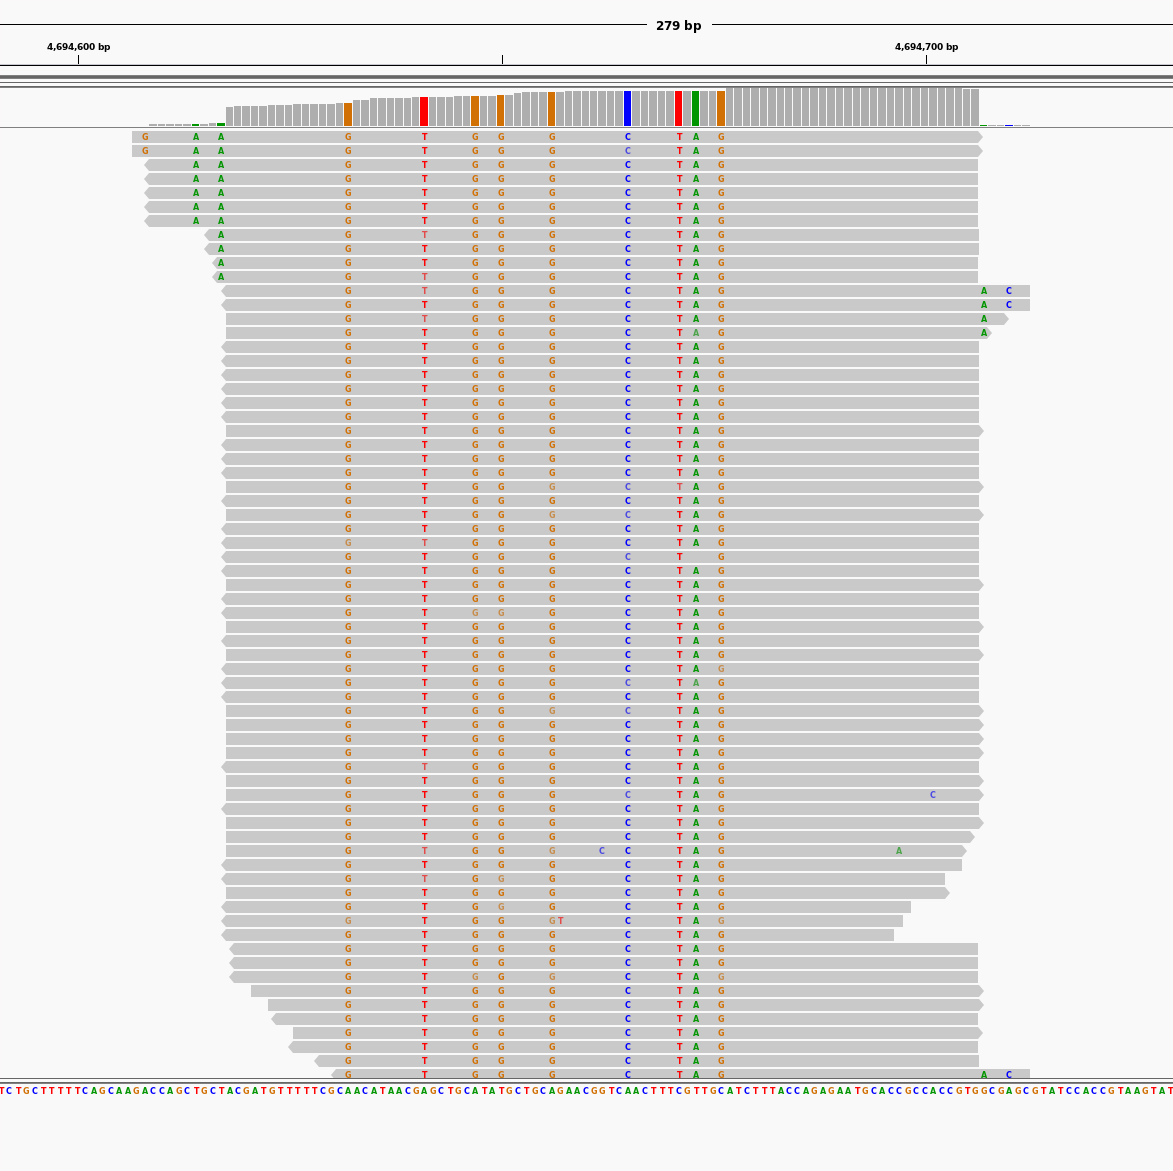
\includegraphics[width=0.35\textheight]{bacillus_reads.png}
\caption{Alignment of short reads from pEU23\_OXA to the \textit{Bacillus cereus}. The reads mapped with a few SNPs which are colored. The reads also did not overlap.}
\label{figure:bacillus_reads}
\end{figure}


\subsection{Growth curves and injected concentrations}
\begin{figure}
	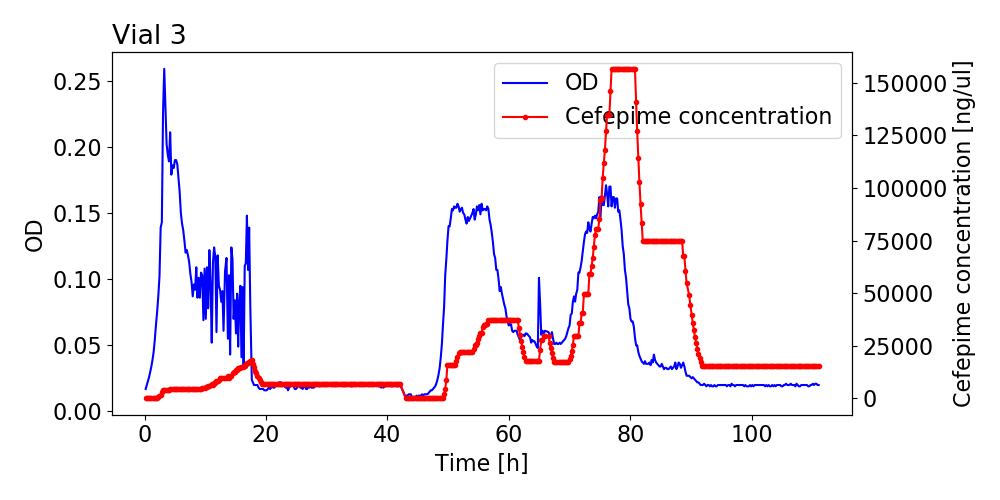
\includegraphics[width=0.5\textwidth]{01_vial_3.png}
	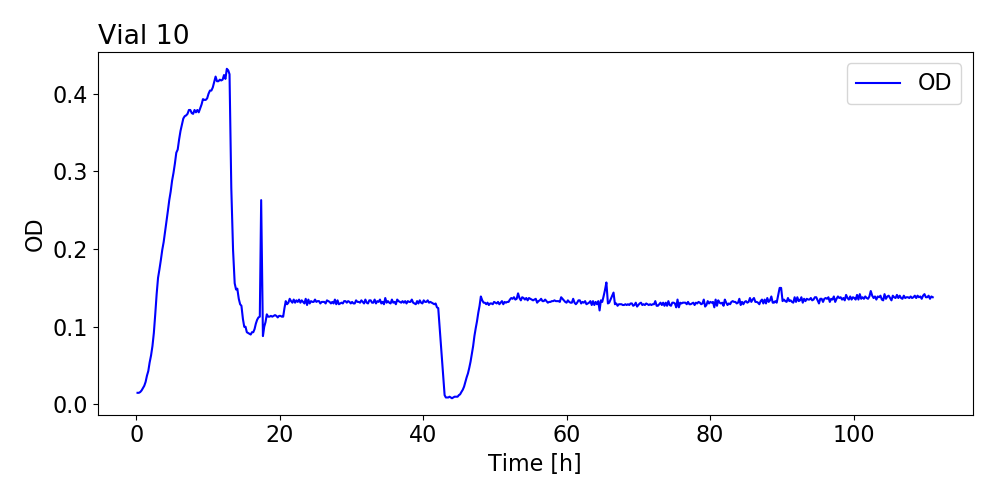
\includegraphics[width=0.5\textwidth]{01_vial_10.png}
	\caption{Growth curves and cefepime concentration in the vials which were not contaminated from experiment 01.}
	\label{figure:01_vials}
\end{figure}

\begin{figure}	
	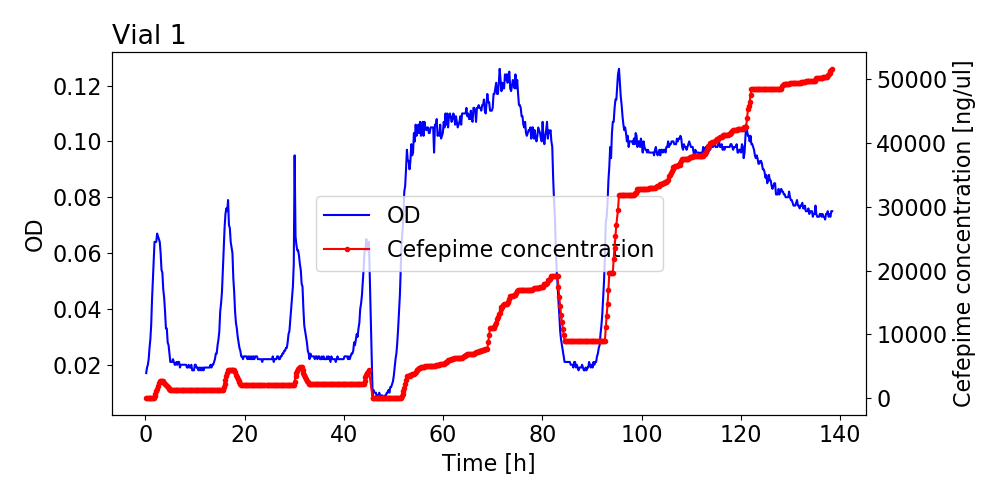
\includegraphics[width=0.5\textwidth]{02_vial_1.png}
	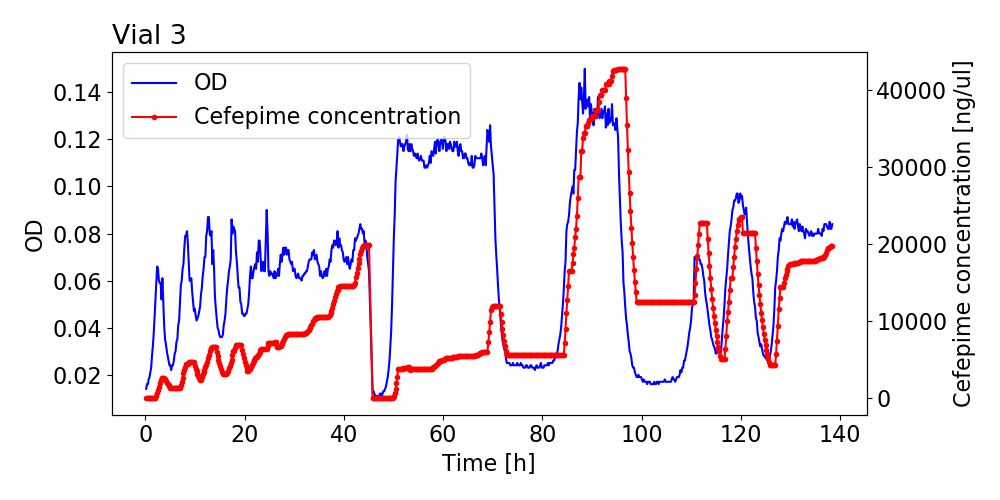
\includegraphics[width=0.5\textwidth]{02_vial_3.png}
	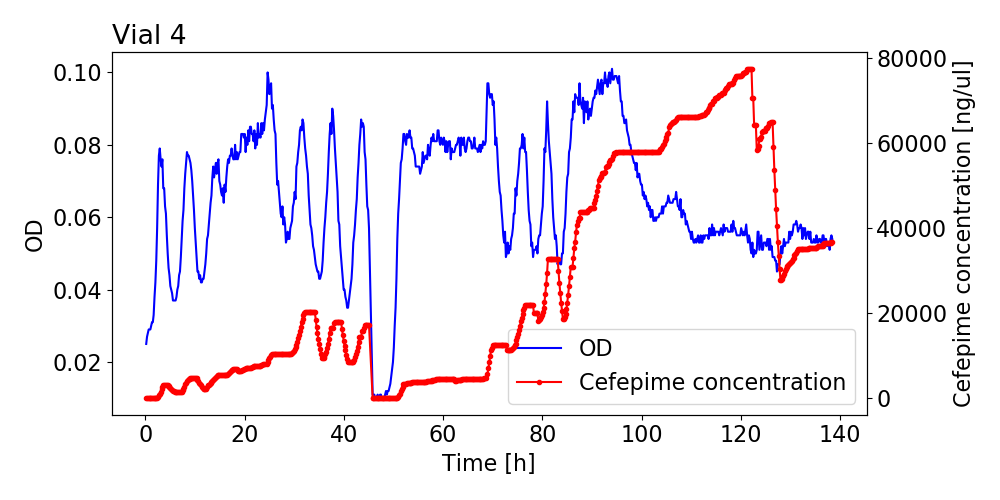
\includegraphics[width=0.5\textwidth]{02_vial_4.png}
	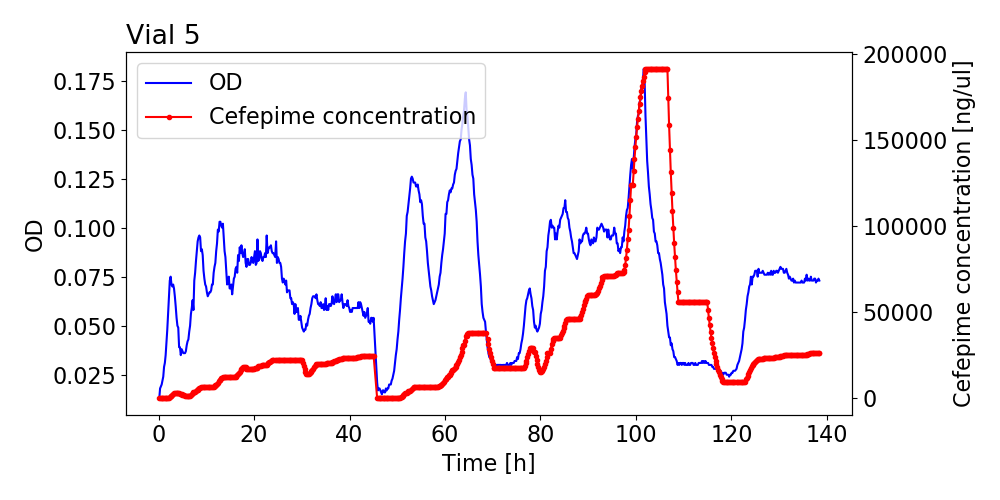
\includegraphics[width=0.5\textwidth]{02_vial_5.png}	
	\caption{Growth curves and cefepime concentration in the vials which were not contaminated from experiment 02.}
	\label{figure:02_vials}
\end{figure}
We recorded the growth curves and stored the cefepime concentrations of every vial during the entire experiment time of both experiments. This allows us to evaluate how well the implemented feedback algorithm reacted to the change of growth. Figure \ref{figure:01_vials} and Figure \ref{figure:02_vials} show the recorded ODs and the cefepime concentration in the vials from the morbidostat experiment 01 (Figure \ref{figure:01_vials}) and 02 (Figure \ref{figure:02_vials}). From both experiments only the vials with no contamination are shown. After 45 hours 200 \textmu L of the cell suspensions were transferred into a new vial with 18 mL diluted media. This is causing the abrupt drop of ODs. In vial 3 from the 01 experiment the OD measurements were very noisy at the beginning which was caused by an air cone coming from high stirring with the magnetic stirrer. After 20 hours the stirring was reduced which eliminated the noise. For vial 10 the mode was set to record growth rate instead of fixed OD. The mode was changed to fixed OD after 15 hours. 
In general the feedback worked really well. The left Figure \ref{figure:vial_3_area} shows the first 45 hours for vial 3 from experiment 02. Drug injection took place after the drug\_dilution\_threshold was reached. After that the cefepime concentration was continuously increased until the cells started to die. The cefepime concentration which was necessary to kill the majority of the cells was stored. Then the feedback diluted the cultures with media until half of the deadly concentration was reached. After that no injections took place until the culture started to grow again. As a result of the feedback the OD was steady but the cefepime concentration was continuously increased. The deadly cefepime concentration after 40 hours of culturing was already four fold higher than at the beginning. 
\begin{figure}
	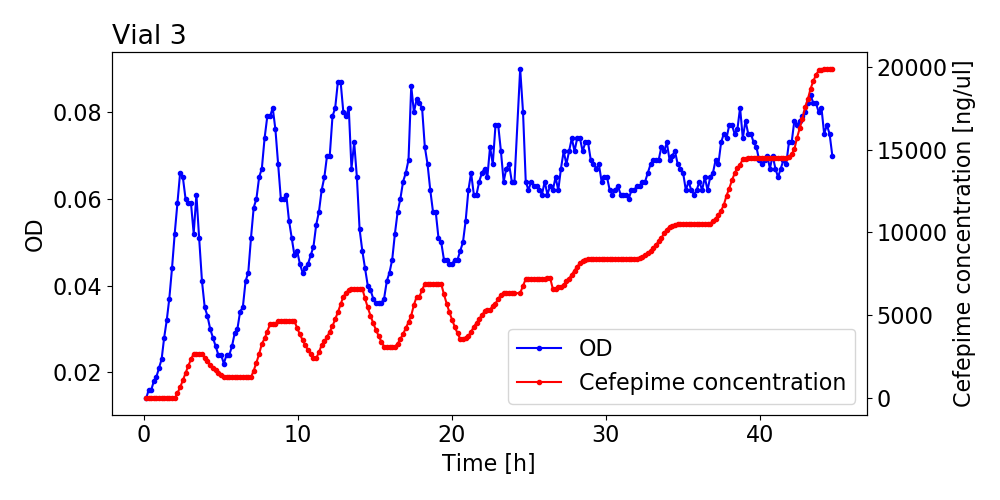
\includegraphics[width=0.5\textwidth]{vial_3_area.png}
	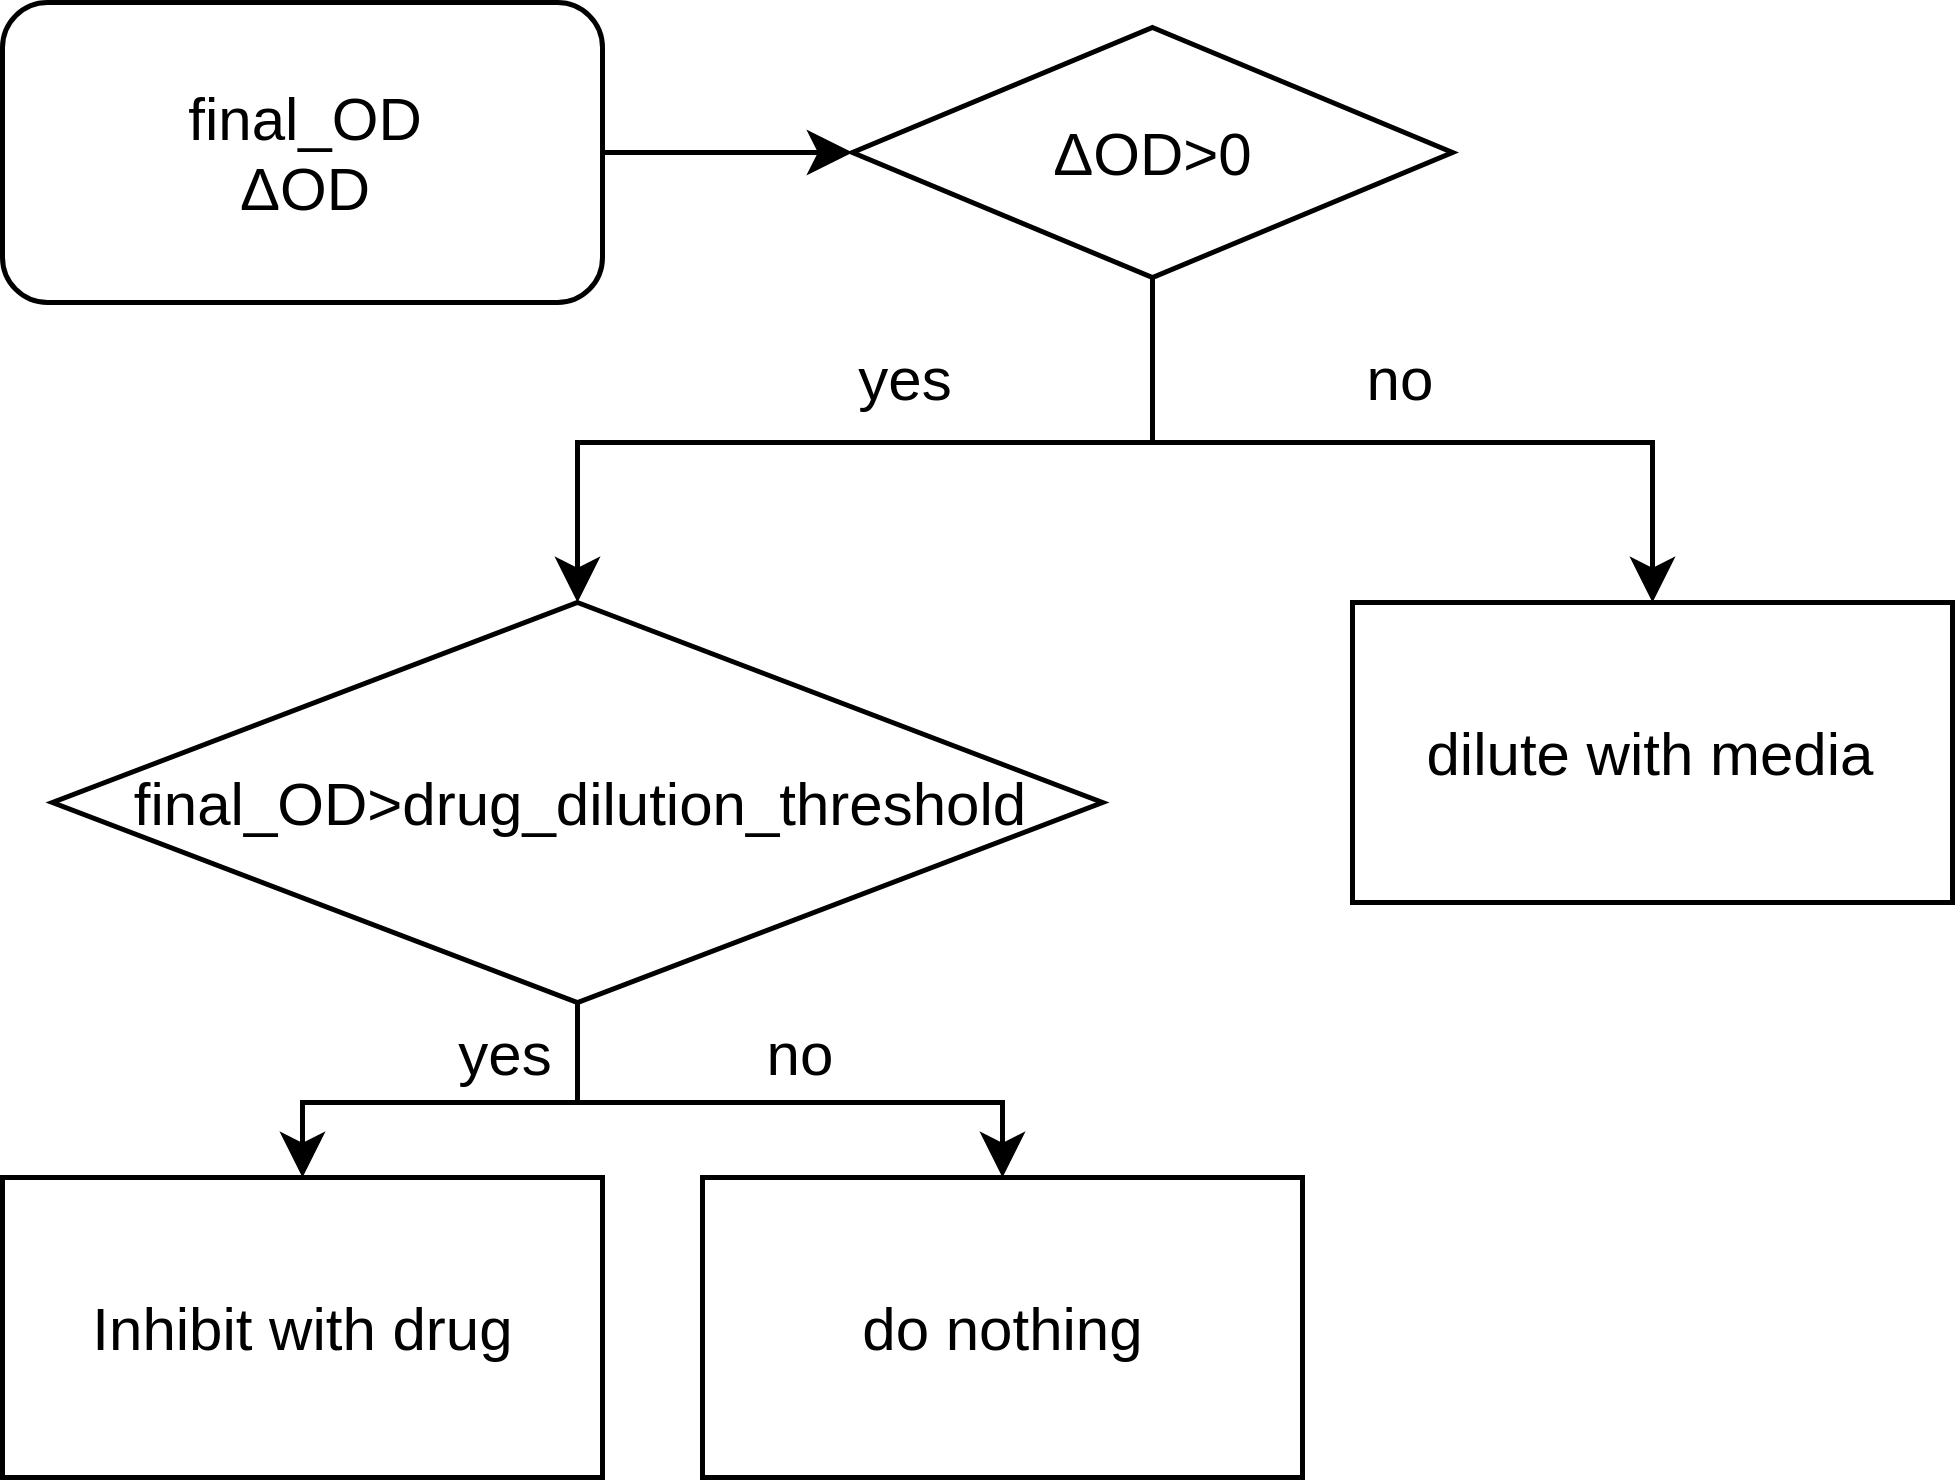
\includegraphics[width=0.5\textwidth]{feedback.png}
	\caption{Left: First 45 hours from vial 3 of experiment 02. Right: Feedback algorithm deciding over drug injection.}
	\label{figure:vial_3_area}
\end{figure}
\subsection{MIC of the strains used for culturing with the morbidostat}
To confirm emerged resistance we determined the MIC of cefepime of the morbidostat samples and the stocks of the strains.
The MICs of the strains before culturing with the morbidostat are shown in Table \ref{table:mics_finish}. In Table \ref{table:mics_finish} the MIC are shown for the samples of the last sample day of the experiment 01 and 02. It is very clear that culturing with the morbidostat increased the resistance. In three cases the increase was over 100 fold. The sample of vial 10 from experiment 01 shows the same MIC as before culturing with the morbidostat. This is as expected, since this vial was cultured with the fixed\_OD mode and no antibiotic pressure was applied.  
\begin{table}
	\begin{tabular}{|ll|}
		\hline
		Strain & MIC of cefepime [\textmu g/mL] \\ \hline
		pEU22  & 8   \\ \hline
		pEU23  & 4   \\ \hline
		pEU26  & 4   \\ \hline
	\end{tabular}
	\quad
	\begin{tabular}{|lll|}
		\hline
		Experiment & Vial & MIC of cefepime [\textmu g/mL] \\ \hline
		01         & 3    & 512                            \\ \hline
		01         & 10   & 4                              \\ \hline
		02         & 1    & 128                            \\ \hline
		02         & 3    & 512                            \\ \hline
		02         & 4    & 512                            \\ \hline
		02         & 5    & 256                            \\ \hline
	\end{tabular}
	\caption{Left Table: MICs of the strains used for the experiment 01 and 02. Right Table: MICs of the samples from the last sample day of the experiment 01 and 02.}
	\label{table:mics_finish}
\end{table}
\subsection{SNPs of experiment 01}
After analyzing the contamination and proving the increase of resistance after culturing with the morbidostat, we present the SNPs which we identified in the samples of the morbidostat. Sample 0 is always the stocked strain before culturing with which the morbidostat was started. The genome of sample 0 is always used as a reference. With this reference we identified SNPs in the samples with evolved resistance applying the same criteria as for the isolate series sampled from patients. We only show vials and samples with no contamination.
\subsubsection{Vial 3}
Even though the MCI of the sample from vial 3 increased over 100 fold, compared to the MIC determined before culturing with the morbidostat, no SNPs were found. 
\subsubsection{Vial 10}
Vial 10 was cultured with the fixed OD mode. The MIC remained the same before and after culturing with the morbidostat. We were still able to identify two SNPs which are shown in Table \ref{table:01_10} with their annotation in Table \ref{table:01_10_ann}.
\begin{table}
	\begin{tabularx}{\linewidth}{|cccLL|}
		\hline
		\#SNP & Contig & Position & \multicolumn{2}{l|}{Nucleotide in Sample:} \\
		&        &          & 0         & \multicolumn{1}{l|}{1}    \\ \hline
		1 & 0 & 3403729 & G & C \\ \hline
	\end{tabularx}
	\caption{SNPs in the samples of vial 10 experiment 01.}
	\label{table:01_10}
\end{table} 
\begin{table}
	\begin{tabularx}{\linewidth}{|ccLLcc|}
		\hline
		\#SNP & Gene          & Product                           & Type and position & \multicolumn{2}{l|}{Amino acid Sample:} \\
		&               &                                   &                   & 0                  & 1                  \\ \hline
	1 & \textit{tomB\_1} & Hha toxicity modulator TomB & Missense, 43 & I & V \\ \hline
	
	\end{tabularx}
	\caption{Genes affected by the SNPs found in the samples of vial 10 experiment 02.}
	\label{table:01_10_ann}
\end{table}
\subsection{SNPs of experiment 02}
\subsubsection{Vial 1}
No SNPs were found in the sample of vial 1, even though the vial was cultured in the continuous mode and the MIC increased over 100 fold. 
\subsubsection{Vial 3}
One SNP was found in the samples of vial 3 which is shown in Table \ref{table:3_02}. Interestingly this mutation affects the kanamycin resistance gene of the vector. The change of amino acid caused by the SNP is shown in Table \ref{table:02_3_ann}.
\begin{table}
	\begin{tabularx}{\linewidth}{|cccLL|}
		\hline
		\#SNP & Contig & Position & \multicolumn{2}{l|}{Nucleotide in Sample:} \\
		&        &          & 0         & \multicolumn{1}{l|}{1}    \\ \hline
		1 & 1 & 4290 & G & T \\ \hline
	\end{tabularx}
	\caption{Positions of SNPs in the samples of vial 3 experiment 02.}
	\label{table:3_02}
\end{table} 
\begin{table}
	\begin{tabularx}{\linewidth}{|ccLLcc|}
		\hline
		\#SNP & Gene          & Product                           & Type and position & \multicolumn{2}{l|}{Amino acid Sample:} \\
		&               &                                   &                   & 0                  & 1                  \\ \hline
		1 & \textit{neoR/kanR} & Kanamycin resistance & Missense, 204 & G & V \\ \hline
		
	\end{tabularx}
	\caption{Genes affected by the SNPs found in the samples of vial 3 experiment 02.}
	\label{table:02_3_ann}
\end{table}
\subsubsection{Vial 4}
Two SNPs were found for the samples of vial 4 shown in Table \ref{table:02_v4} and the affected genes in Table \ref{table:02_v4_ann}.
\begin{table}
	\begin{tabularx}{\linewidth}{|cccLLL|}
		\hline
		\#SNP & Contig & Position & \multicolumn{3}{l|}{Nucleotide in Sample:} \\
		&        &          & 0     & 1     & \multicolumn{1}{l|}{2}    \\ \hline
		1 & 1 & 2526   & T & T & A \\ \hline
		2 & 0 & 347328 & C & C & T \\ \hline
	\end{tabularx}
	\caption{Positions of SNPs in the samples of vial 4 experiment 02.}
	\label{table:02_v4}
\end{table}

\begin{table}
	\begin{tabularx}{\linewidth}{|ccLLccc|}
		\hline
		\#SNP & Gene          & Product                                  & Type and position in gene      & \multicolumn{3}{l|}{Amino acid in Sample:} \\
		&               &                                          &                        & 0   & 1               & 2               \\ \hline
		1 & \textit{bla}  & Beta-lactamase CTX-M-1                  & Missense, 289 & V & V & D \\ \hline
		2 & \textit{ompR} & Transcriptional regulatory protein OmpR & Nonsense, 67  & R & R & * \\ \hline
	\end{tabularx}
	\caption{Genes affected by the SNPs found in the samples of vial 4 experiment 02. The star in sample 2 stands for a stop codon.}
	\label{table:02_v4_ann}
\end{table}
\subsubsection{Vial 5}
Three SNPs were found for the samples of vial 5. SNPs are shown Table \ref{table:02_v5}, annotations in Table \ref{table:02_v5_ann}.
\begin{table}
	\begin{tabularx}{\linewidth}{|cccLLL|}
		\hline
		\#SNP & Contig & Position & \multicolumn{3}{l|}{Nucleotide in Sample:} \\
		&        &          & 0     & 1     & \multicolumn{1}{l|}{2}    \\ \hline
		1 & 0 & 1570984 & C & C & T \\ \hline
		2 & 0 & 668881  & A & T & A \\ \hline
		3 & 0 & 2898640 & G & G & - \\ \hline
	\end{tabularx}
	\caption{Positions of SNPs in the samples of vial 5 experiment 02.}
	\label{table:02_v5}
\end{table}

\begin{table}
	\begin{tabularx}{\linewidth}{|ccLLccc|}
		\hline
		\#SNP & Gene          & Product                                  & Type and position in gene      & \multicolumn{3}{l|}{Amino acid in Sample:} \\
		&               &                                          &                        & 0   & 1               & 2               \\ \hline
		1 & \textit{ompC\_1} & Outer membrane protein C         & Silent, 8              & L & L & L \\ \hline
		2 & \textit{rpoD}    & RNA polymerase sigma factor RpoD & Missense, 594             & L & Q & L \\ \hline
		3 & \textit{ompF}    & Outer membrane protein F         & Frameshift, 319 & G & G & A \\ \hline
	\end{tabularx}
	\caption{Genes affected by the SNPs found in the samples of vial 5 experiment 02.}
	\label{table:02_v5_ann}
\end{table}
